\section{Auswertung}
\label{sec:Auswertung}
\subsection{Fourier-Synthese}
Mit den berechneten Verhältnissen ergeben sich beim Einstellen der Rechteckspannung die in Abbildung \ref{fig:recht} dargestellte Funktion.

\begin{figure}[H]
  \centering
  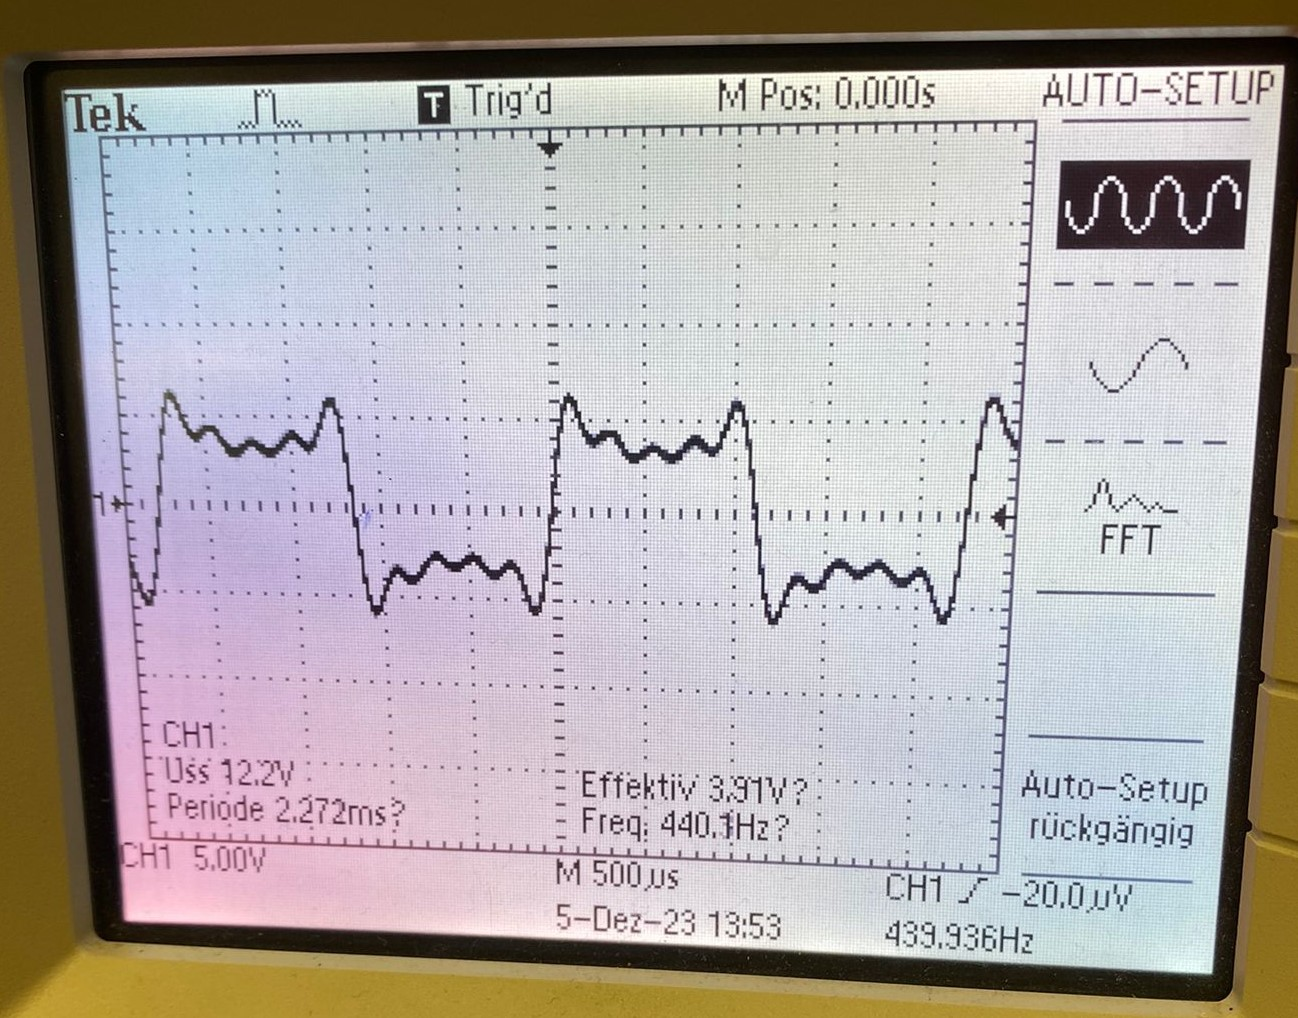
\includegraphics[height=7cm]{Bilder/recht.jpg}
  \caption{Ergebnis der Rechteckspannung mit Fourier-Synthese.}
  \label{fig:recht}
\end{figure}

Für die Dreieckspannung wurde die Funktion in Abbildung \ref{fig:drei} erreicht.

\begin{figure}[H]
  \centering
  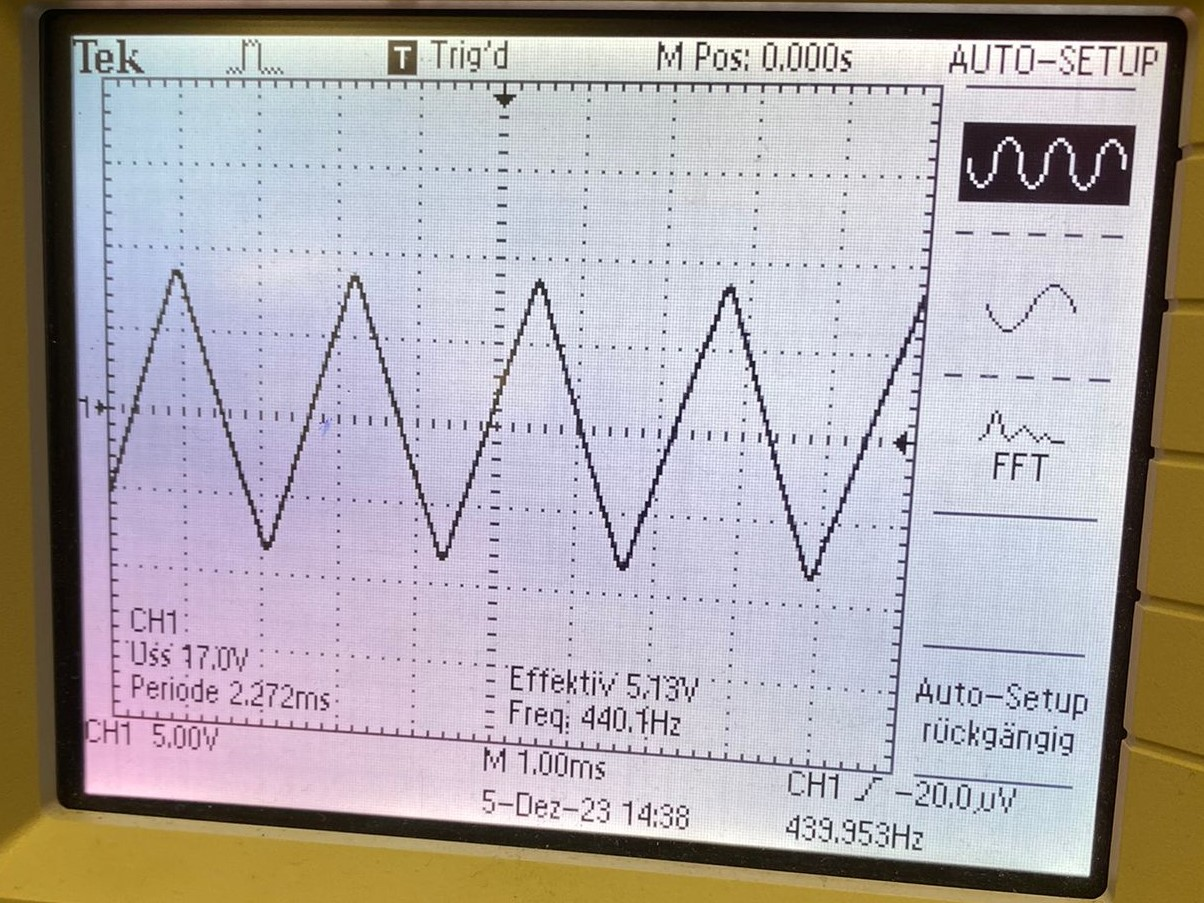
\includegraphics[height=7cm]{Bilder/drei.jpg}
  \caption{Ergebnis der Dreieckspannung mit Fourier-Synthese.}
  \label{fig:drei}
\end{figure}


Die Fourier-Synthese ergibt bei der Sägezahnspannung den Plot in Abbildung \ref{fig:säge}.
\begin{figure}[H]
  \centering
  \includegraphics[height=7cm]{Bilder/säge.jpg}
  \caption{Ergebnis der Sägezahnspannung mit Fourier-Synthese.}
  \label{fig:säge}
\end{figure}

\subsection{Fourier-Analyse}
Für die Fourer-Analyse wurden die Werte in Tabelle \ref{tab:tabelle4} gemessen.

\begin{table}[htbp]
  \centering
  \caption{Messwerte der Amplituden in Abhängigkeit zur Frequenz von der Rechteckspannung, der Sägezahnspannung und der Dreieckspannung.}
  \label{tab:tabelle4}
  \begin{minipage}[t]{0.3\linewidth}
  \begin{tblr}[t]{
    colspec={S[table-format=3.0] S[table-format=2.1]},
    row{1}={guard, mode=math},
    }
    \toprule
      f \mathbin{/} \unit{\kilo\hertz} &  A_{R} \mathbin{/} \unit{\decibel} \\
    \midrule
      10  &    39.0 \\
      30  &    29.4 \\
      50  &    25.0 \\
      70  &    22.2 \\
      90  &    20.2 \\
      110 &    18.2 \\
      130 &    17.0 \\
      150 &    15.8 \\
      170 &    14.6 \\
      190 &    13.8 \\ 
    \bottomrule
  \end{tblr}
  
\end{minipage}
\hfill
\begin{minipage}[t]{0.3\linewidth}
  \begin{tblr}[t]{
    colspec={S[table-format=3.0] S[table-format=2.1]},
    row{1}={guard, mode=math},
    }
    \toprule
    f \mathbin{/} \unit{\kilo\hertz} &  A_{S} \mathbin{/} \unit{\decibel} \\ 
    \midrule
    10  &    33.0 \\
    20  &    27.0 \\
    30  &    23.4 \\
    40  &    21.0 \\
    50  &    19.0 \\
    60  &    17.4 \\
    70  &    16.2 \\
    80  &    15.0 \\
    90  &    14.2 \\
    100 &    13.0 \\
    \bottomrule
  \end{tblr}

\end{minipage}
\hfill
  \begin{minipage}[t]{0.3\linewidth}
  \begin{tblr}[t]{
    colspec={S[table-format=2.0] S[table-format=2.2]},
    row{1}={guard, mode=math},
    }
    \toprule
      f \mathbin{/} \unit{\kilo\hertz} &  A_{D} \mathbin{/} \unit{\decibel} \\
    \midrule
    10 &     35.00 \\
    30 &     15.80 \\
    50 &      7.41 \\
    70 &      1.01 \\
    \bottomrule
  \end{tblr}
  
\end{minipage}
\hfill
\end{table}

Die Werte für die Amplituden werden mit der Formel
\begin{equation*}
  \unit{\volt}=10^{\frac{\unit{\decibel}}{20}}
\end{equation*}
von Dezibel in Volt umgerechnet.
Diese werden dann in Abbildung \ref{fig:plot1} geplottet.
Dazu werden noch die Theoriewerte geplottet die mit den Formeln \ref{eqn:b_recht}, \ref{eqn:b_drei} und \ref{eqn:b_säge} berechnet werden.

\begin{figure}[H]
  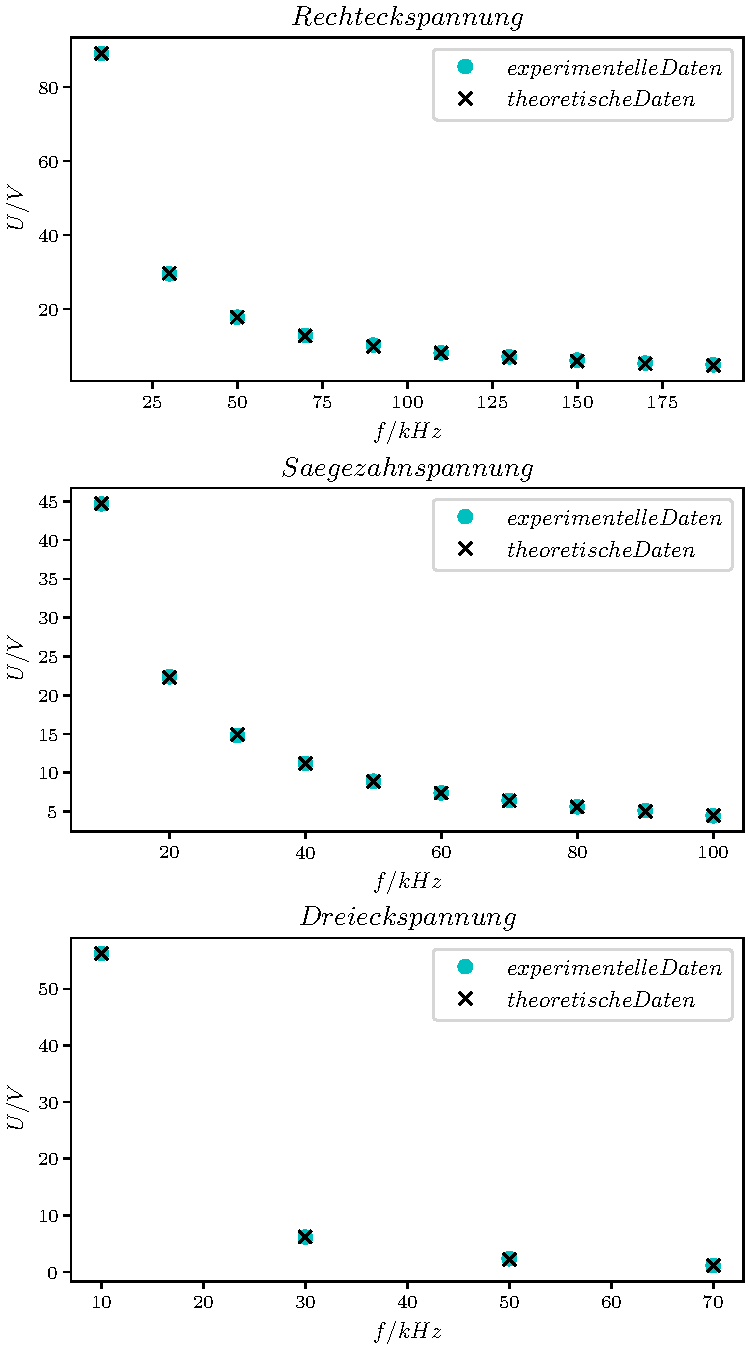
\includegraphics[width=\textwidth]{plot1.pdf}
  \label{fig:plot1}
\caption{Hier sind die Graphen von Experimental- und Theoriewert der Amplituden in Volt gegen die Frequenz im Kilohertz aufgetragen.}
\end{figure}


